\documentclass{report}

\usepackage{booktabs}
\usepackage[utf8]{inputenc}
\usepackage{graphicx}
\usepackage{pgfplots}
\DeclareUnicodeCharacter{2212}{−}
\usepgfplotslibrary{groupplots,dateplot}
\usetikzlibrary{patterns,shapes.arrows}
\pgfplotsset{compat=newest}

\title{MATH 610 PA 1 Report}
\author{Jordan Hoffart}
\date{\today}
\begin{document}
\maketitle

\chapter*{Problem 1}
\section*{$S = 100$}
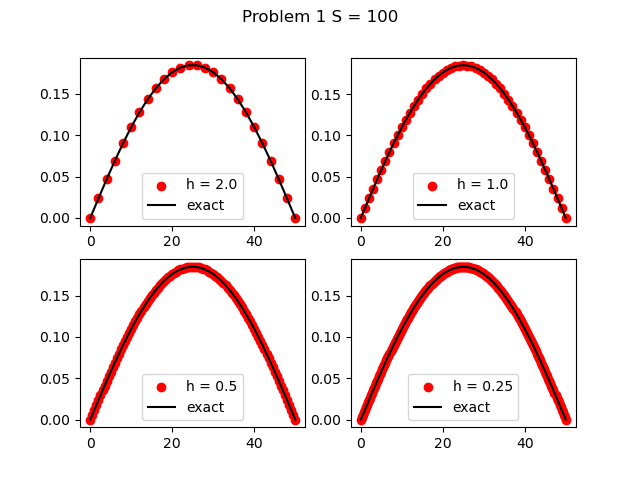
\includegraphics[width=\textwidth]{../data/problem-1/problem_1_S_100.png}
\begin{center}
	\begin{tabular}{rrrrrrr}
\toprule
mesh size & L2 error & H1 error & Linf error & L2 rate & H1 rate & Linf rate \\
\midrule
2.00E+00 & 1.34E-03 & 2.50E-03 & 3.55E-04 & 0.00E+00 & 0.00E+00 & 0.00E+00 \\
1.00E+00 & 3.35E-04 & 1.11E-03 & 8.87E-05 & 2.00E+00 & 1.17E+00 & 2.00E+00 \\
5.00E-01 & 8.37E-05 & 5.36E-04 & 2.22E-05 & 2.00E+00 & 1.05E+00 & 2.00E+00 \\
2.50E-01 & 2.09E-05 & 2.65E-04 & 5.55E-06 & 2.00E+00 & 1.01E+00 & 2.00E+00 \\
\bottomrule
\end{tabular}

\end{center}
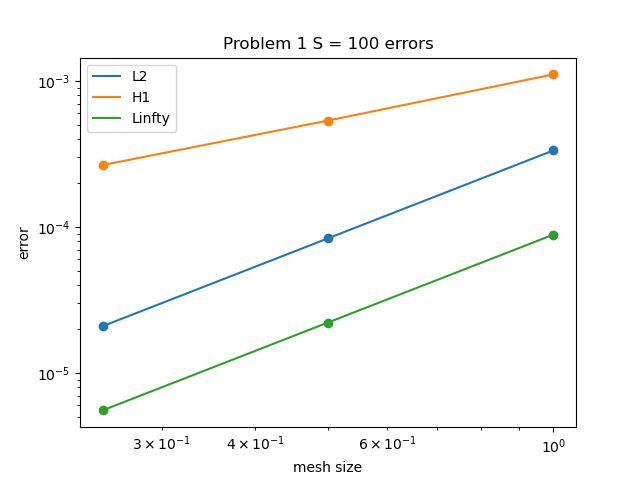
\includegraphics[width=\textwidth]{../data/problem-1/problem_1_S_100_errors.png}
\section*{$S = 1000$}
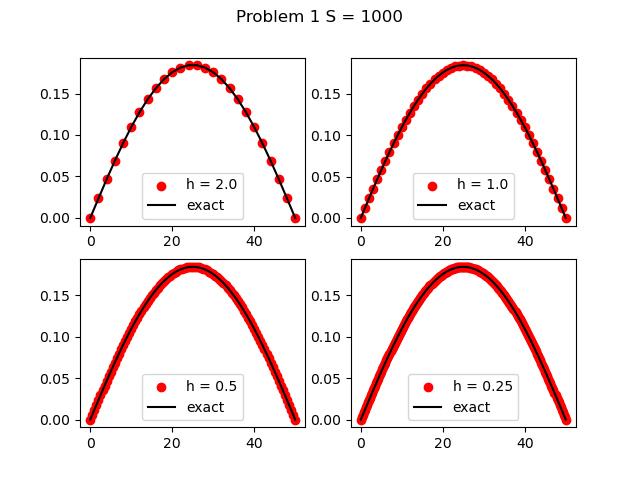
\includegraphics[width=\textwidth]{../data/problem-1/problem_1_S_1000.png}
\begin{center}
	\input{../data/problem-1/problem_1_S_1000_errors.tex}
\end{center}
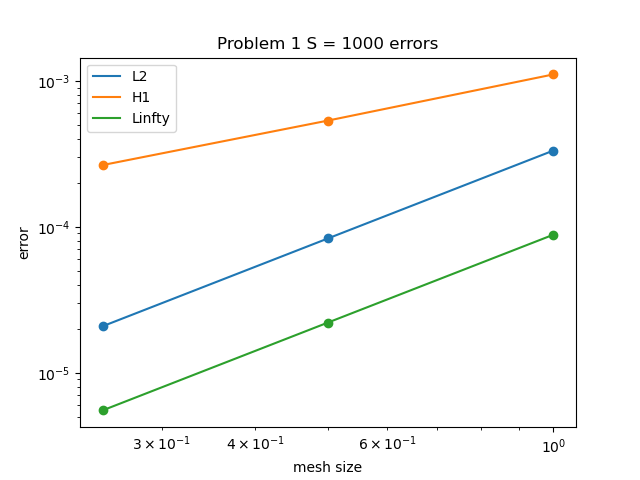
\includegraphics[width=\textwidth]{../data/problem-1/problem_1_S_1000_errors.png}
\section*{$S = 10000$}
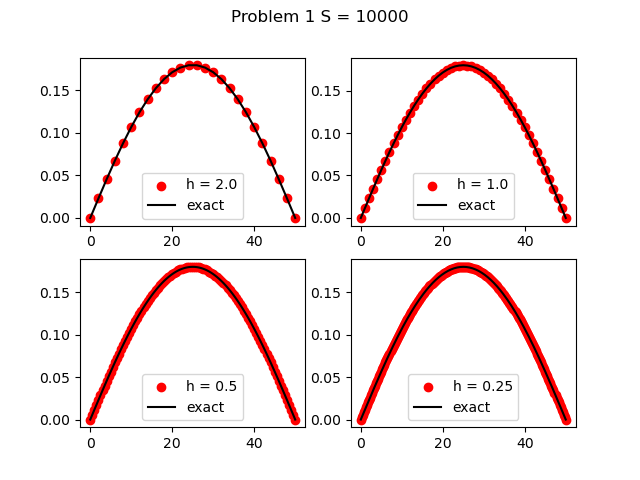
\includegraphics[width=\textwidth]{../data/problem-1/problem_1_S_10000.png}
\begin{center}
	\begin{tabular}{rrrrrrr}
\toprule
mesh size & L2 error & H1 error & Linf error & L2 rate & H1 rate & Linf rate \\
\midrule
2.00E+00 & 1.27E-03 & 2.42E-03 & 3.38E-04 & 0.00E+00 & 0.00E+00 & 0.00E+00 \\
1.00E+00 & 3.18E-04 & 1.08E-03 & 8.45E-05 & 2.00E+00 & 1.17E+00 & 2.00E+00 \\
5.00E-01 & 7.95E-05 & 5.21E-04 & 2.11E-05 & 2.00E+00 & 1.05E+00 & 2.00E+00 \\
2.50E-01 & 1.99E-05 & 2.58E-04 & 5.29E-06 & 2.00E+00 & 1.01E+00 & 2.00E+00 \\
\bottomrule
\end{tabular}

\end{center}
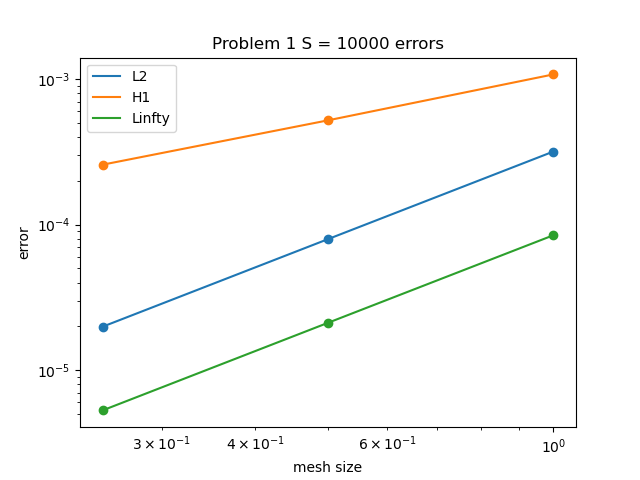
\includegraphics[width=\textwidth]{../data/problem-1/problem_1_S_10000_errors.png}

\chapter*{Problem 2}
\section*{$S = 100$}
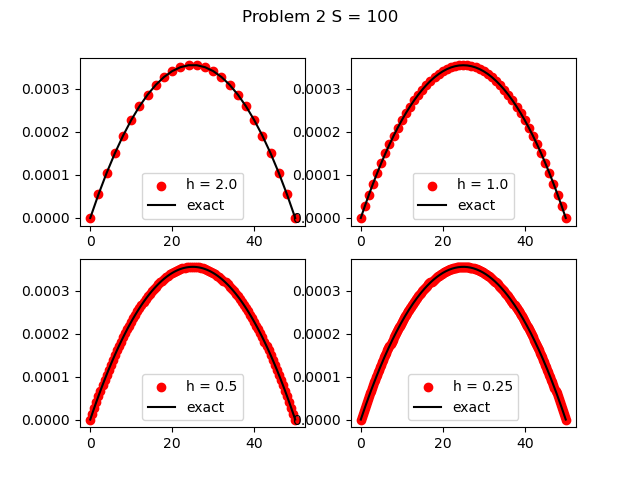
\includegraphics[width=\textwidth]{../data/problem-2/problem_2_S_100.png}
\begin{center}
	\begin{tabular}{rrrrrrr}
\toprule
mesh size & L2 error & H1 error & Linf error & L2 rate & H1 rate & Linf rate \\
\midrule
2.00E+00 & 2.93E-06 & 5.49E-06 & 5.68E-07 & 0.00E+00 & 0.00E+00 & 0.00E+00 \\
1.00E+00 & 7.33E-07 & 2.43E-06 & 1.42E-07 & 2.00E+00 & 1.17E+00 & 2.00E+00 \\
5.00E-01 & 1.83E-07 & 1.17E-06 & 3.55E-08 & 2.00E+00 & 1.05E+00 & 2.00E+00 \\
2.50E-01 & 4.58E-08 & 5.82E-07 & 8.88E-09 & 2.00E+00 & 1.01E+00 & 2.00E+00 \\
\bottomrule
\end{tabular}

\end{center}
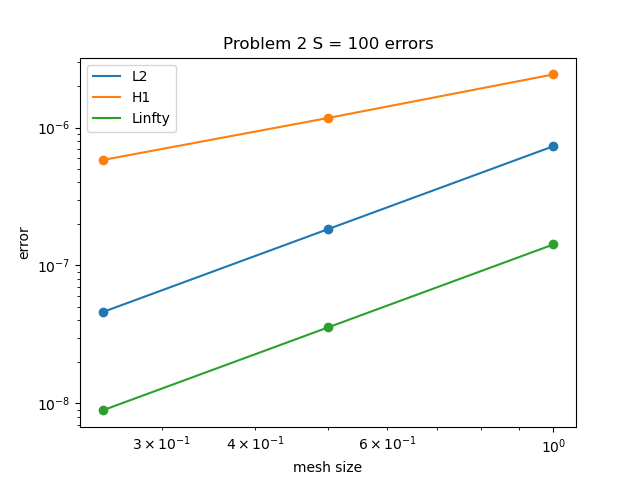
\includegraphics[width=\textwidth]{../data/problem-2/problem_2_S_100_errors.png}
\section*{$S = 1000$}
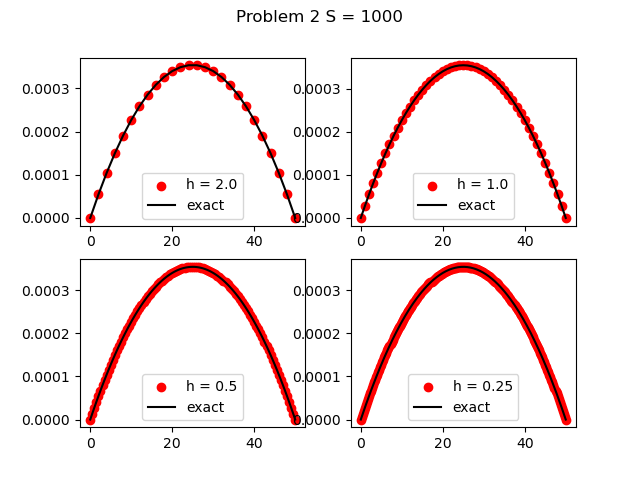
\includegraphics[width=\textwidth]{../data/problem-2/problem_2_S_1000.png}
\begin{center}
	\begin{tabular}{rrrrrrr}
\toprule
mesh size & L2 error & H1 error & Linf error & L2 rate & H1 rate & Linf rate \\
\midrule
2.00E+00 & 2.92E-06 & 5.47E-06 & 5.68E-07 & 0.00E+00 & 0.00E+00 & 0.00E+00 \\
1.00E+00 & 7.30E-07 & 2.43E-06 & 1.42E-07 & 2.00E+00 & 1.17E+00 & 2.00E+00 \\
5.00E-01 & 1.83E-07 & 1.17E-06 & 3.55E-08 & 2.00E+00 & 1.05E+00 & 2.00E+00 \\
2.50E-01 & 4.56E-08 & 5.80E-07 & 8.88E-09 & 2.00E+00 & 1.01E+00 & 2.00E+00 \\
\bottomrule
\end{tabular}

\end{center}
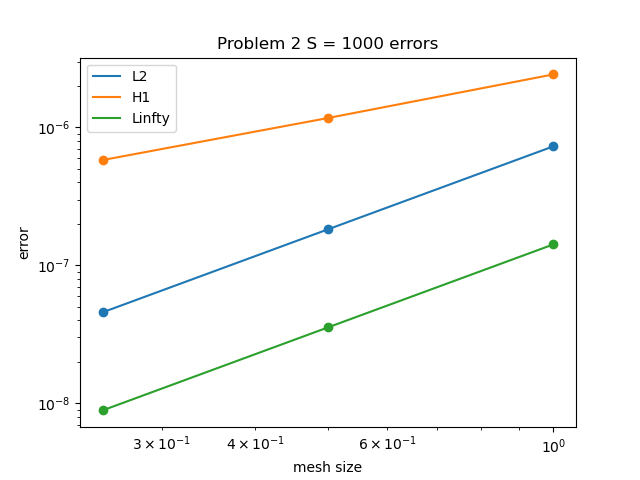
\includegraphics[width=\textwidth]{../data/problem-2/problem_2_S_1000_errors.png}
\section*{$S = 10000$}
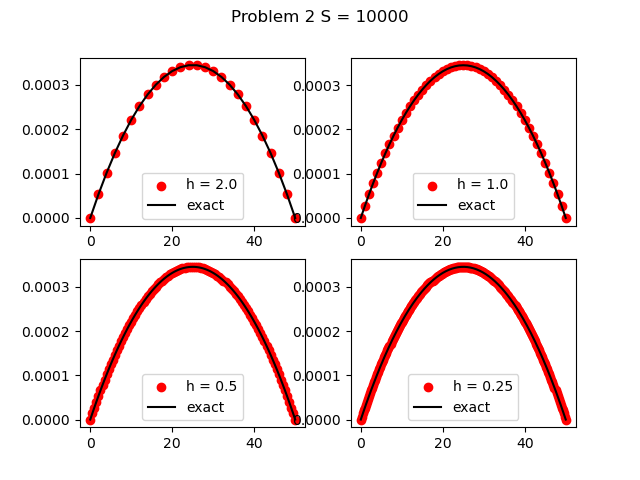
\includegraphics[width=\textwidth]{../data/problem-2/problem_2_S_10000.png}
\begin{center}
	\begin{tabular}{rrrrrrr}
\toprule
mesh size & L2 error & H1 error & Linf error & L2 rate & H1 rate & Linf rate \\
\midrule
2.00E+00 & 2.81E-06 & 5.33E-06 & 5.66E-07 & 0.00E+00 & 0.00E+00 & 0.00E+00 \\
1.00E+00 & 7.03E-07 & 2.37E-06 & 1.42E-07 & 2.00E+00 & 1.17E+00 & 2.00E+00 \\
5.00E-01 & 1.76E-07 & 1.15E-06 & 3.55E-08 & 2.00E+00 & 1.05E+00 & 2.00E+00 \\
2.50E-01 & 4.39E-08 & 5.68E-07 & 8.87E-09 & 2.00E+00 & 1.01E+00 & 2.00E+00 \\
\bottomrule
\end{tabular}

\end{center}
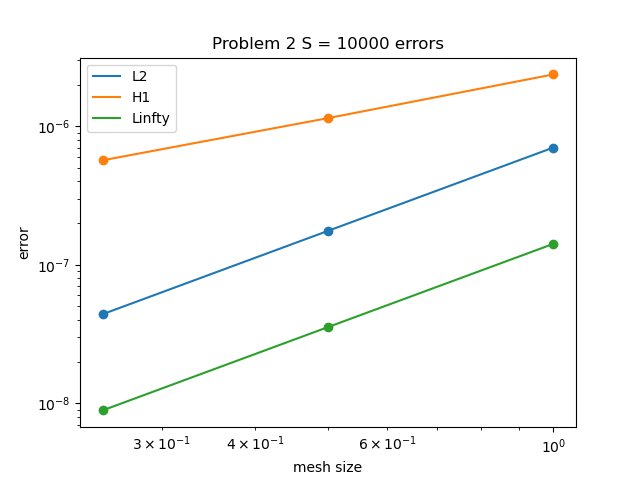
\includegraphics[width=\textwidth]{../data/problem-2/problem_2_S_10000_errors.png}

\chapter*{Problem 3}
\section*{Non-constant rhs}
\subsection*{$S = 100$}
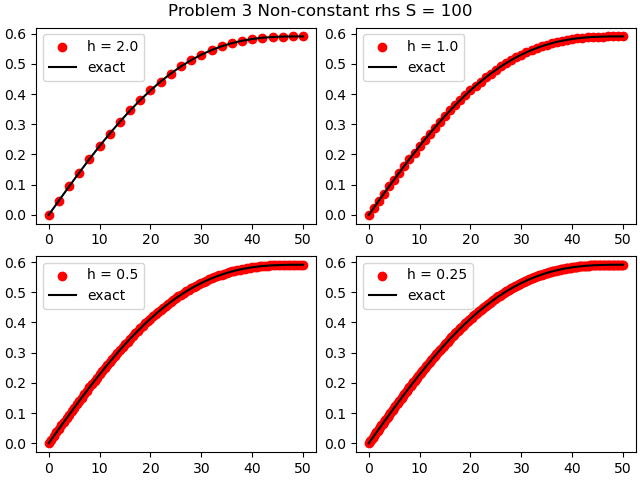
\includegraphics[width=\textwidth]{../data/problem-3/problem_3_non_constant_rhs_S_100.png}
\begin{center}
	\begin{tabular}{rrrrrrr}
\toprule
mesh size & L2 error & H1 error & Linf error & L2 rate & H1 rate & Linf rate \\
\midrule
2.00E+00 & 1.34E-03 & 2.50E-03 & 3.55E-04 & 0.00E+00 & 0.00E+00 & 0.00E+00 \\
1.00E+00 & 3.34E-04 & 1.11E-03 & 8.86E-05 & 2.00E+00 & 1.17E+00 & 2.00E+00 \\
5.00E-01 & 8.36E-05 & 5.35E-04 & 2.22E-05 & 2.00E+00 & 1.05E+00 & 2.00E+00 \\
2.50E-01 & 2.09E-05 & 2.65E-04 & 5.54E-06 & 2.00E+00 & 1.01E+00 & 2.00E+00 \\
\bottomrule
\end{tabular}

\end{center}
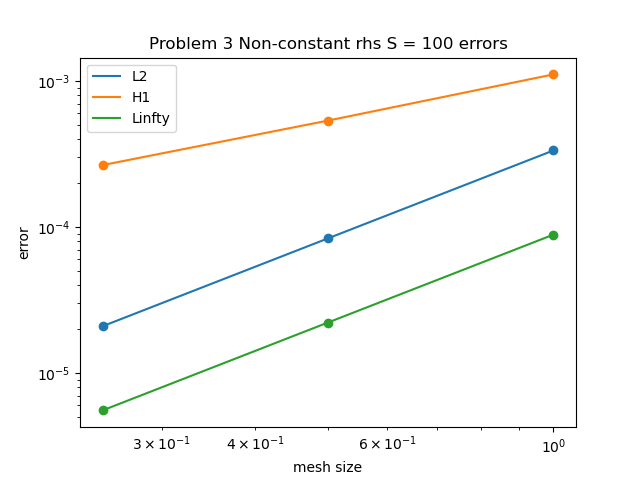
\includegraphics[width=\textwidth]{../data/problem-3/problem_3_non_constant_rhs_S_100_errors.png}

\subsection*{$S = 1000$}
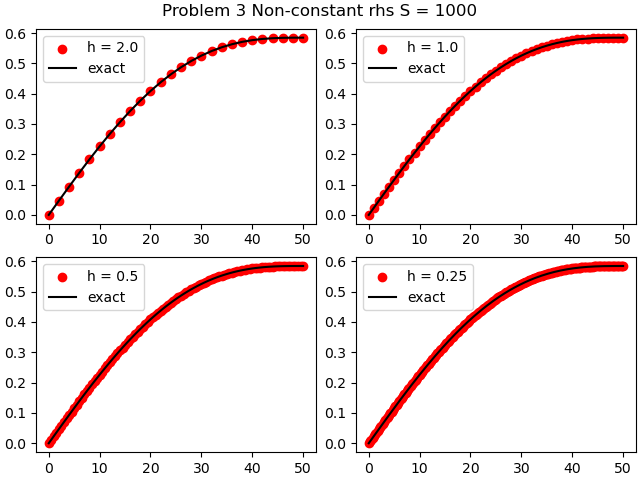
\includegraphics[width=\textwidth]{../data/problem-3/problem_3_non_constant_rhs_S_1000.png}
\begin{center}
	\begin{tabular}{rrrrrrr}
\toprule
mesh size & L2 error & H1 error & Linf error & L2 rate & H1 rate & Linf rate \\
\midrule
2.00E+00 & 1.32E-03 & 2.48E-03 & 3.51E-04 & 0.00E+00 & 0.00E+00 & 0.00E+00 \\
1.00E+00 & 3.29E-04 & 1.10E-03 & 8.76E-05 & 2.00E+00 & 1.17E+00 & 2.00E+00 \\
5.00E-01 & 8.24E-05 & 5.31E-04 & 2.19E-05 & 2.00E+00 & 1.05E+00 & 2.00E+00 \\
2.50E-01 & 2.06E-05 & 2.63E-04 & 5.48E-06 & 2.00E+00 & 1.01E+00 & 2.00E+00 \\
\bottomrule
\end{tabular}

\end{center}
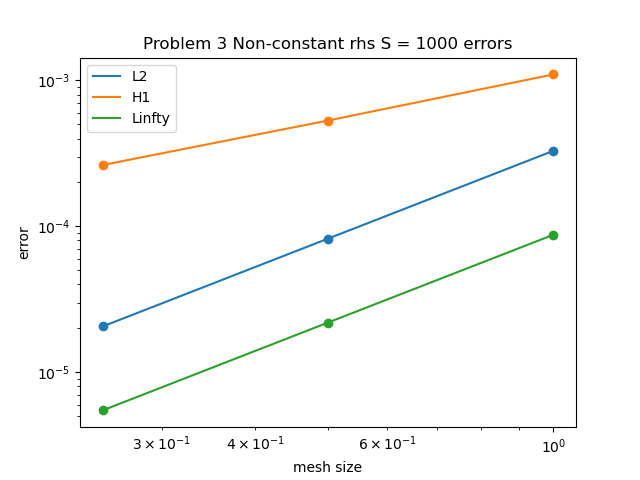
\includegraphics[width=\textwidth]{../data/problem-3/problem_3_non_constant_rhs_S_1000_errors.png}

\subsection*{$S = 10000$}
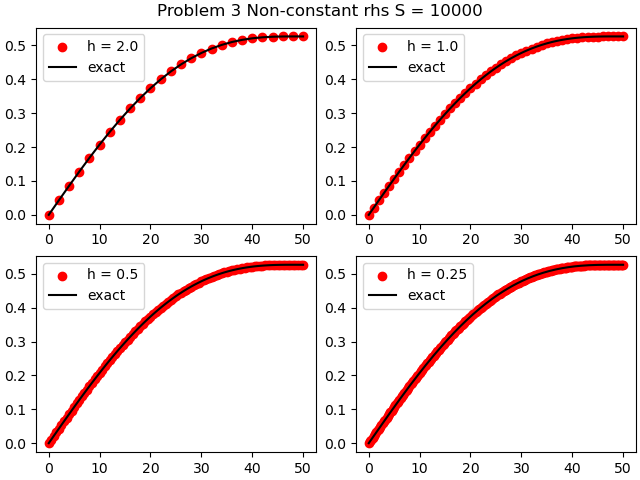
\includegraphics[width=\textwidth]{../data/problem-3/problem_3_non_constant_rhs_S_10000.png}
\begin{center}
	\begin{tabular}{rrrrrrr}
\toprule
mesh size & L2 error & H1 error & Linf error & L2 rate & H1 rate & Linf rate \\
\midrule
2.00E+00 & 1.16E-03 & 2.27E-03 & 3.16E-04 & 0.00E+00 & 0.00E+00 & 0.00E+00 \\
1.00E+00 & 2.90E-04 & 1.02E-03 & 7.90E-05 & 2.00E+00 & 1.16E+00 & 2.00E+00 \\
5.00E-01 & 7.24E-05 & 4.93E-04 & 1.98E-05 & 2.00E+00 & 1.05E+00 & 2.00E+00 \\
2.50E-01 & 1.81E-05 & 2.45E-04 & 4.94E-06 & 2.00E+00 & 1.01E+00 & 2.00E+00 \\
\bottomrule
\end{tabular}

\end{center}
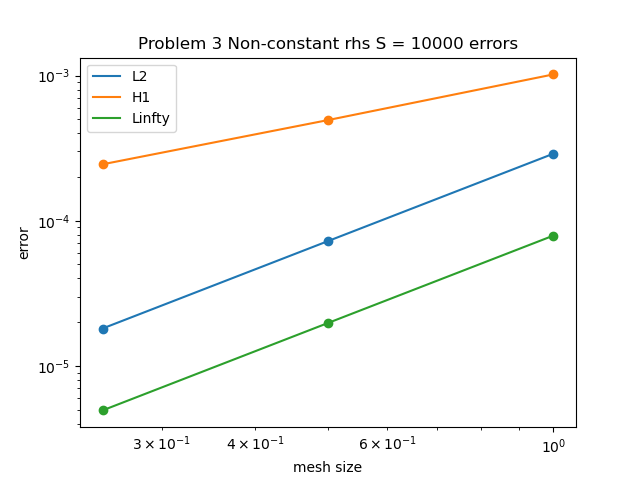
\includegraphics[width=\textwidth]{../data/problem-3/problem_3_non_constant_rhs_S_10000_errors.png}

\section*{Constant rhs}
\subsection*{$S = 100$}
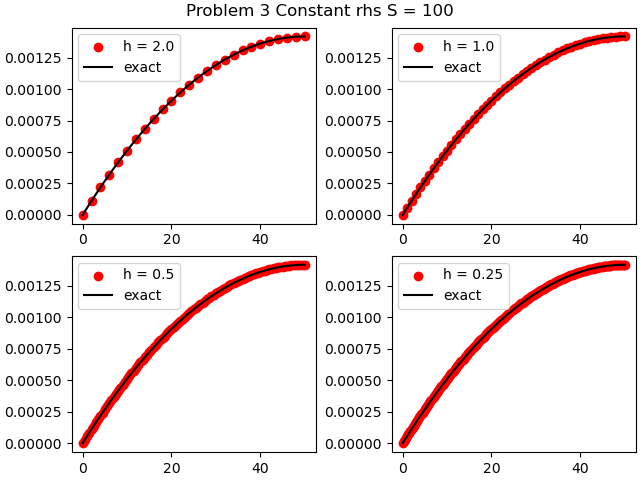
\includegraphics[width=\textwidth]{../data/problem-3/problem_3_constant_rhs_S_100.png}
\begin{center}
	\input{../data/problem-3/problem_3_constant_rhs_S_100_errors.tex}
\end{center}
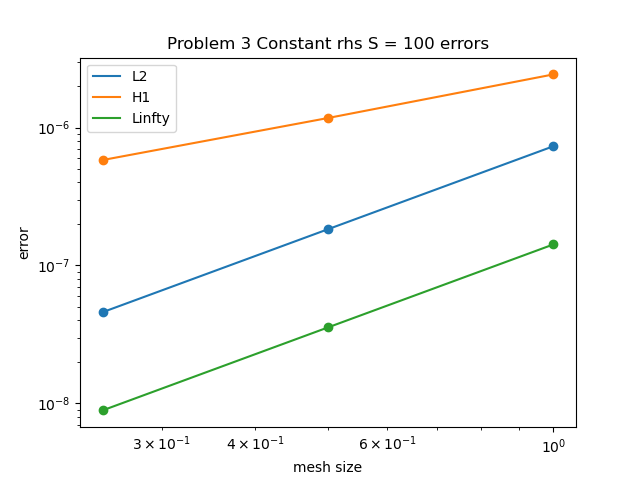
\includegraphics[width=\textwidth]{../data/problem-3/problem_3_constant_rhs_S_100_errors.png}

\subsection*{$S = 1000$}
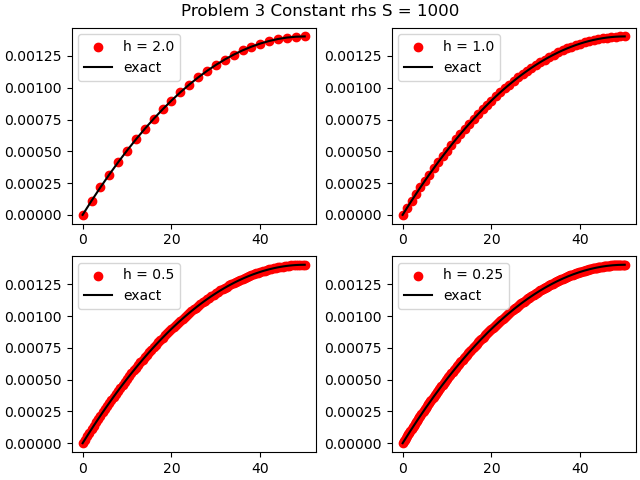
\includegraphics[width=\textwidth]{../data/problem-3/problem_3_constant_rhs_S_1000.png}
\begin{center}
	\input{../data/problem-3/problem_3_constant_rhs_S_1000_errors.tex}
\end{center}
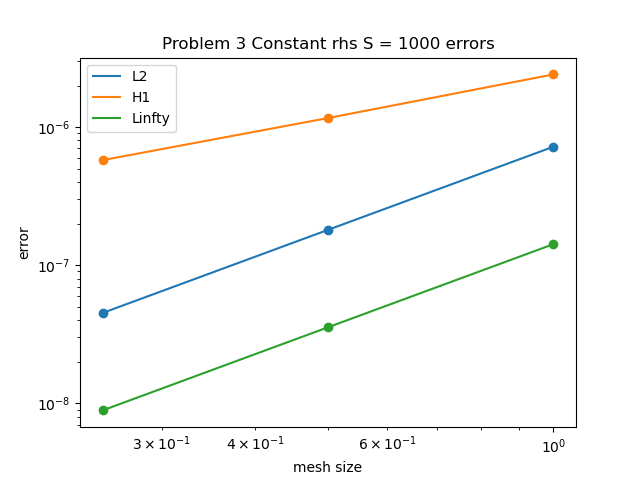
\includegraphics[width=\textwidth]{../data/problem-3/problem_3_constant_rhs_S_1000_errors.png}

\subsection*{$S = 10000$}
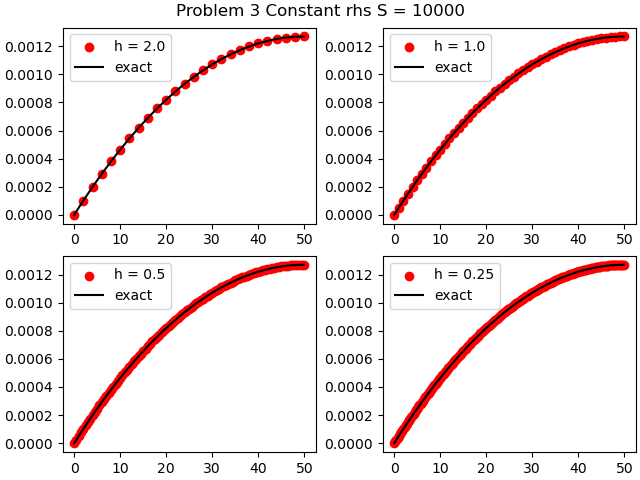
\includegraphics[width=\textwidth]{../data/problem-3/problem_3_constant_rhs_S_10000.png}
\begin{center}
	\begin{tabular}{rrrrrrr}
\toprule
mesh size & L2 error & H1 error & Linf error & L2 rate & H1 rate & Linf rate \\
\midrule
2.00E+00 & 2.51E-06 & 4.93E-06 & 5.64E-07 & 0.00E+00 & 0.00E+00 & 0.00E+00 \\
1.00E+00 & 6.27E-07 & 2.21E-06 & 1.41E-07 & 2.00E+00 & 1.16E+00 & 1.99E+00 \\
5.00E-01 & 1.57E-07 & 1.07E-06 & 3.54E-08 & 2.00E+00 & 1.04E+00 & 2.00E+00 \\
2.50E-01 & 3.92E-08 & 5.32E-07 & 8.87E-09 & 2.00E+00 & 1.01E+00 & 2.00E+00 \\
\bottomrule
\end{tabular}

\end{center}
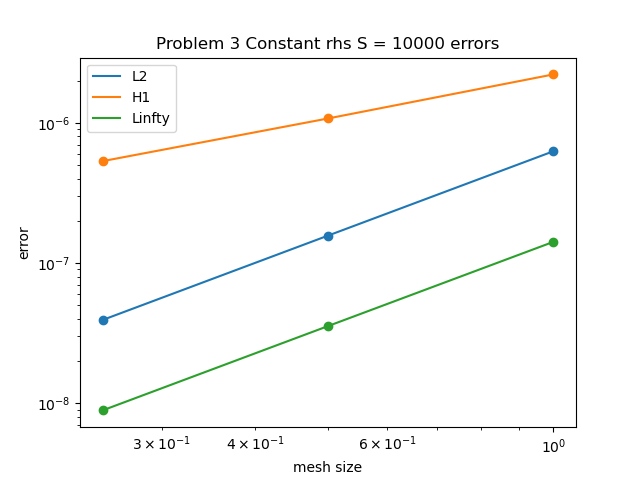
\includegraphics[width=\textwidth]{../data/problem-3/problem_3_constant_rhs_S_10000_errors.png}

\chapter*{Problem 4}
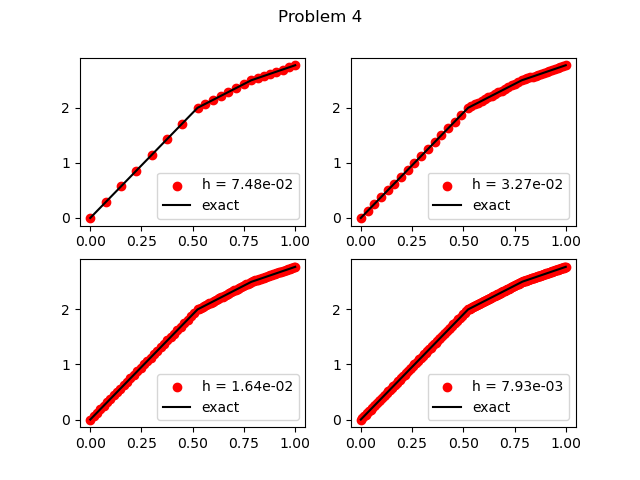
\includegraphics[width=\textwidth]{../data/problem-4/problem_4.png}
\begin{center}
	\input{../data/problem-4/problem_4_errors.tex}
\end{center}
\end{document}
